\documentclass[12pt,a4]{article}
\usepackage{booktabs}
\usepackage[left=1.8cm,right=1.8cm,top=32mm,columnsep=20pt]{geometry}
\usepackage{fontspec}
\usepackage[spanish, es-tabla, es-nodecimaldot]{babel}
\usepackage{amsmath, amsfonts}
\usepackage{float}
\usepackage{graphicx}
\usepackage{hyperref}
\usepackage{siunitx}
\usepackage{multicol}
\usepackage{tocloft}
\usepackage[sorting=none]{biblatex}
\addbibresource{main.bib}

\title{
    \vspace*{1cm}
    \textbf{\LARGE Análisis experimental de la ley de escala\\[2pt]
    en bollos de papel con distintos gramajes}\\[1.2cm]
    \large Federico Tomás Moroni \quad Nicolás Ezequiel López \quad Gaia Tornielli\\[0.4cm]
    \normalsize Universidad de San Andrés\\
    Ingeniería en Inteligencia Artificial\\
    I208 — Física I\\[0.2cm]
    \texttt{ftmoroni@udesa.edu.ar} \quad \texttt{nelopez@udesa.edu.ar} \quad \texttt{gtornielli@udesa.edu.ar}\\[1cm]
    \normalsize \textbf{1er semestre de 2025}
    \vspace*{0.5cm}
}
\author{}
\date{}

\begin{document}
\maketitle
\begin{abstract}
En esta práctica se investigó la relación entre el diámetro de los bollos de papel y la masa de la hoja utilizada, explorando una posible ley de escala del tipo \( D = A \cdot M^b \). Se midieron áreas, masas, volúmenes y diámetros para tres tipos de papel con diferentes gramajes, propagando las incertidumbres correspondientes. Se obtuvieron exponentes característicos mediante ajustes logarítmico-logarítmico (log-log) y no lineal. Asimismo, se estimó el gramaje del papel a partir de un ajuste ortogonal. Los resultados muestran que el valor del exponente \( b \) aumenta con el gramaje, lo que sugiere una influencia estructural del material en el proceso de compactación.
\end{abstract}
\newpage
\renewcommand{\cfttoctitlefont}{\Large\bfseries}
\renewcommand{\contentsname}{Contenido}
\setlength{\cftbeforesecskip}{4pt}
\setlength{\cftbeforesubsecskip}{2pt}
\tableofcontents
\newpage

\section{Introducción}

Las leyes de escala, que describen cómo las propiedades de un sistema varían con su tamaño~\cite{clauset}, son fundamentales en diversas áreas de la física. En este trabajo se propone explorar una posible ley de escala en un objeto cotidiano: los bollos de papel. Específicamente, se investiga si el diámetro de estos bollos se relaciona con la masa de la hoja utilizada de manera predecible, y si dicha relación depende del tipo de papel empleado.

Comprender esta relación permite estudiar cómo las propiedades estructurales del papel influyen en el proceso de compactación, conectando fenómenos aparentemente simples con conceptos de geometría, materiales y estadística.

Para abordar esta pregunta, se seleccionaron tres tipos de papel con diferentes gramajes. A partir de hojas de distintos tamaños se formaron bollos de manera manual, midiendo cuidadosamente sus masas y diámetros. 

El presente informe se estructura del siguiente modo: en la próxima sección se detalla el desarrollo experimental, incluyendo los materiales, mediciones e instrumentos utilizados. Luego, se presentan los resultados y se discuten sus implicancias. Finalmente, se expone una síntesis de las conclusiones más relevantes.

\subsection{Marco teórico}

El modelo principal que se busca verificar experimentalmente es una ley de escala entre el diámetro \( D \) de un bollo de papel y la masa \( M \) de la hoja utilizada, mediante la expresión:

\begin{equation}
D = A \cdot M^b
\label{eq:ley_escala}
\end{equation}

donde \( A \) es una constante característica del sistema y \( b \) es el exponente de escala.

Para analizar cuantitativamente las relaciones involucradas, se utilizan los siguientes modelos físicos:

\paragraph{Área del papel.} A partir de las dimensiones de la hoja (largo \( L \) y ancho \( W \)), el área se calcula como:

\begin{equation}
A = L \cdot W
\label{eq:area}
\end{equation}

La incertidumbre asociada, por propagación de errores independientes, se obtiene mediante:

\begin{equation}
\delta A = \sqrt{(W \cdot \delta L)^2 + (L \cdot \delta W)^2}
\label{eq:delta_area}
\end{equation}

\paragraph{Volumen del bollo.} Asumiendo una forma esférica ideal, el volumen del bollo se estima con:

\begin{equation}
V = \frac{4}{3} \pi \left( \frac{D}{2} \right)^3
\label{eq:volumen}
\end{equation}

y su incertidumbre asociada es:

\begin{equation}
\delta V = \frac{\pi D^2}{2} \cdot \delta D
\label{eq:delta_volumen}
\end{equation}

\paragraph{Gramaje del papel.} El gramaje \( G \), definido como la masa por unidad de superficie en g/m\(^2\), se calcula como:

\begin{equation}
G = \frac{10000 \cdot M}{A}
\label{eq:gramaje}
\end{equation}

La incertidumbre se evalúa como:

\begin{equation}
\delta G = G \cdot \sqrt{\left( \frac{\delta M}{M} \right)^2 + \left( \frac{\delta A}{A} \right)^2}
\label{eq:delta_gramaje}
\end{equation}

Estas expresiones permiten estudiar la influencia del tipo de papel en el proceso de arrugamiento, evaluando experimentalmente la validez del modelo de escala planteado.

\bigskip

El objetivo principal de esta práctica es verificar la existencia de una ley de escala del tipo Ec.~\eqref{eq:ley_escala} entre el diámetro del bollo y la masa del papel, así como analizar la variación del exponente \( b \) en función del gramaje. Además, se propone estimar experimentalmente el gramaje mediante un modelo lineal con ajuste ortogonal. 


\section{Desarrollo experimental}

Para llevar a cabo la verificación experimental de la ley de escala, se trabajó con tres tipos de papel: liviano, medio y pesado. En cada caso, se cortaron hojas de diferentes tamaños y se formaron bollos de manera manual, procurando mantener una técnica de compactación lo más constante posible.

Las variables medidas para cada muestra fueron:

\begin{itemize}
    \item Longitud \( L \) y ancho \( W \) de la hoja, mediante una regla milimetrada, con una incertidumbre instrumental de \( \delta L = \delta W = \SI{0.05}{cm} \).
    \item Masa \( M \), con una balanza digital de precisión, con incertidumbre instrumental de \( \delta M = \SI{0.01}{g} \).
    \item Diámetro \( D \) del bollo, usando una regla, repitiendo la medición al menos seis veces por muestra para obtener un valor promedio y su error.
\end{itemize}

El cálculo de las magnitudes derivadas —como el área, volumen y gramaje— se realizó siguiendo las expresiones detalladas en la sección de Marco teórico (ver Ecs.~\eqref{eq:area}–\eqref{eq:delta_gramaje}). Se aplicaron criterios de propagación de incertidumbre para todas las magnitudes calculadas.

Además del análisis manual, se utilizó un script en Python para el procesamiento automatizado de los datos. Este código permitió:

\begin{itemize}
    \item Calcular promedios y errores combinando incertidumbres instrumentales y estadísticas.
    \item Ajustar la ley de potencia \( D = A \cdot M^b \) de forma no lineal y en escala log-log.
    \item Aplicar un ajuste ortogonal por mínimos cuadrados (ODR) para estimar el gramaje a partir del modelo lineal \( M = G \cdot A \).
    \item Generar automáticamente los gráficos presentados en la sección de Resultados.
\end{itemize}

El uso de estas herramientas permitió una mayor rigurosidad y trazabilidad en el análisis, facilitando la validación cruzada entre distintos métodos de ajuste. Todas las funciones empleadas están documentadas y disponibles para su revisión, asegurando transparencia y reproducibilidad de los resultados.

\section{Resultados y análisis}

\subsection{Relación entre diámetro y masa}

Para cada tipo de papel se graficó el diámetro promedio de los bollos en función de su masa (Figura~\ref{fig:diametro_vs_masa}). Aunque la relación no es lineal en escala aritmética, se observa una clara tendencia creciente, lo cual motiva el uso de una ley de escala como la expresada en la Ec.~\eqref{eq:ley_escala}.

\begin{figure}[H]
    \centering
    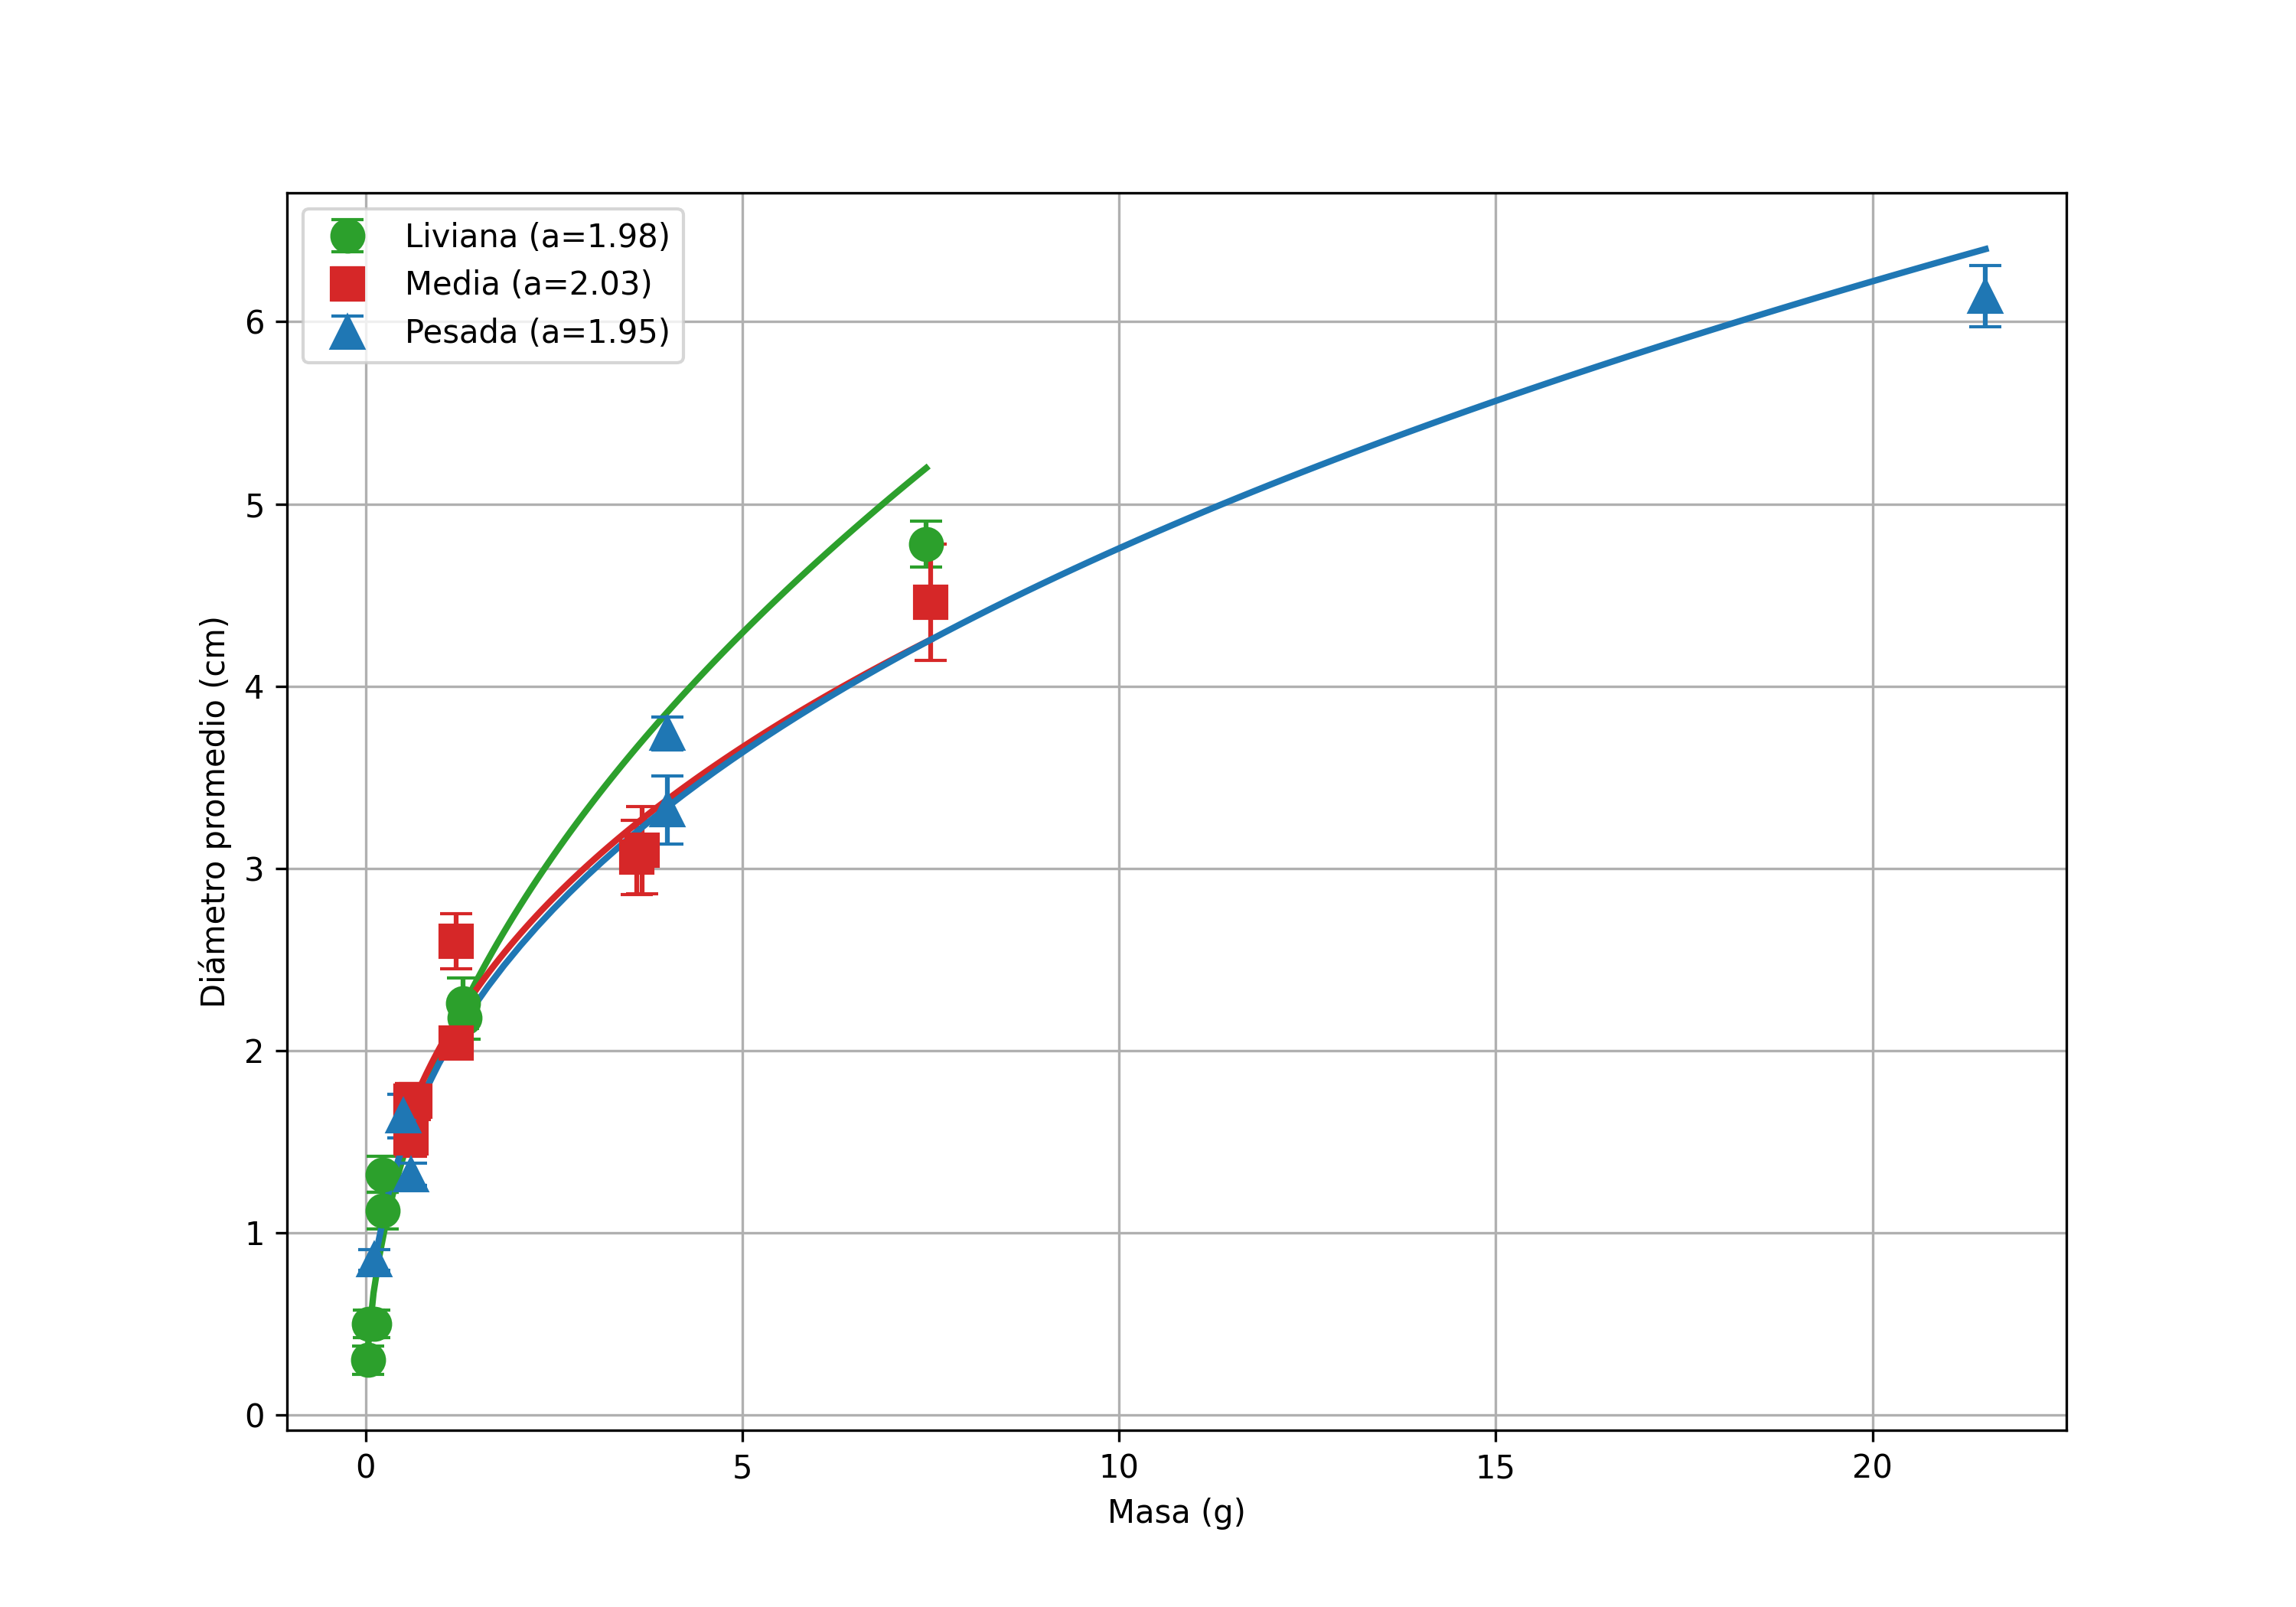
\includegraphics[width=0.45\textwidth]{diametro_vs_masa.png}
    \caption{Diámetro promedio de los bollos en función de la masa, diferenciados por grupo. Las líneas muestran el ajuste no lineal \( D = A \cdot M^b \) realizado con \texttt{curve\_fit}.}
    \label{fig:diametro_vs_masa}
\end{figure}

Por ejemplo, una muestra del grupo medio con un área de \( A = \SI{300}{cm^2} \) y una masa de \( M = \SI{4.9}{g} \), produjo un bollo de diámetro \( D = \SI{4.2}{cm} \), en buena concordancia con la tendencia general observada. En todos los casos, el diámetro se calculó como el promedio de múltiples repeticiones, incorporando tanto el error instrumental como el error estadístico.

Para analizar la ley de escala de manera más rigurosa, se transformaron los datos al espacio logarítmico. La representación log-log (Figura~\ref{fig:loglog}) linealiza el modelo y permite aplicar un ajuste ponderado que ofrece una estimación robusta del exponente \( b \).

\begin{figure}[H]
    \centering
    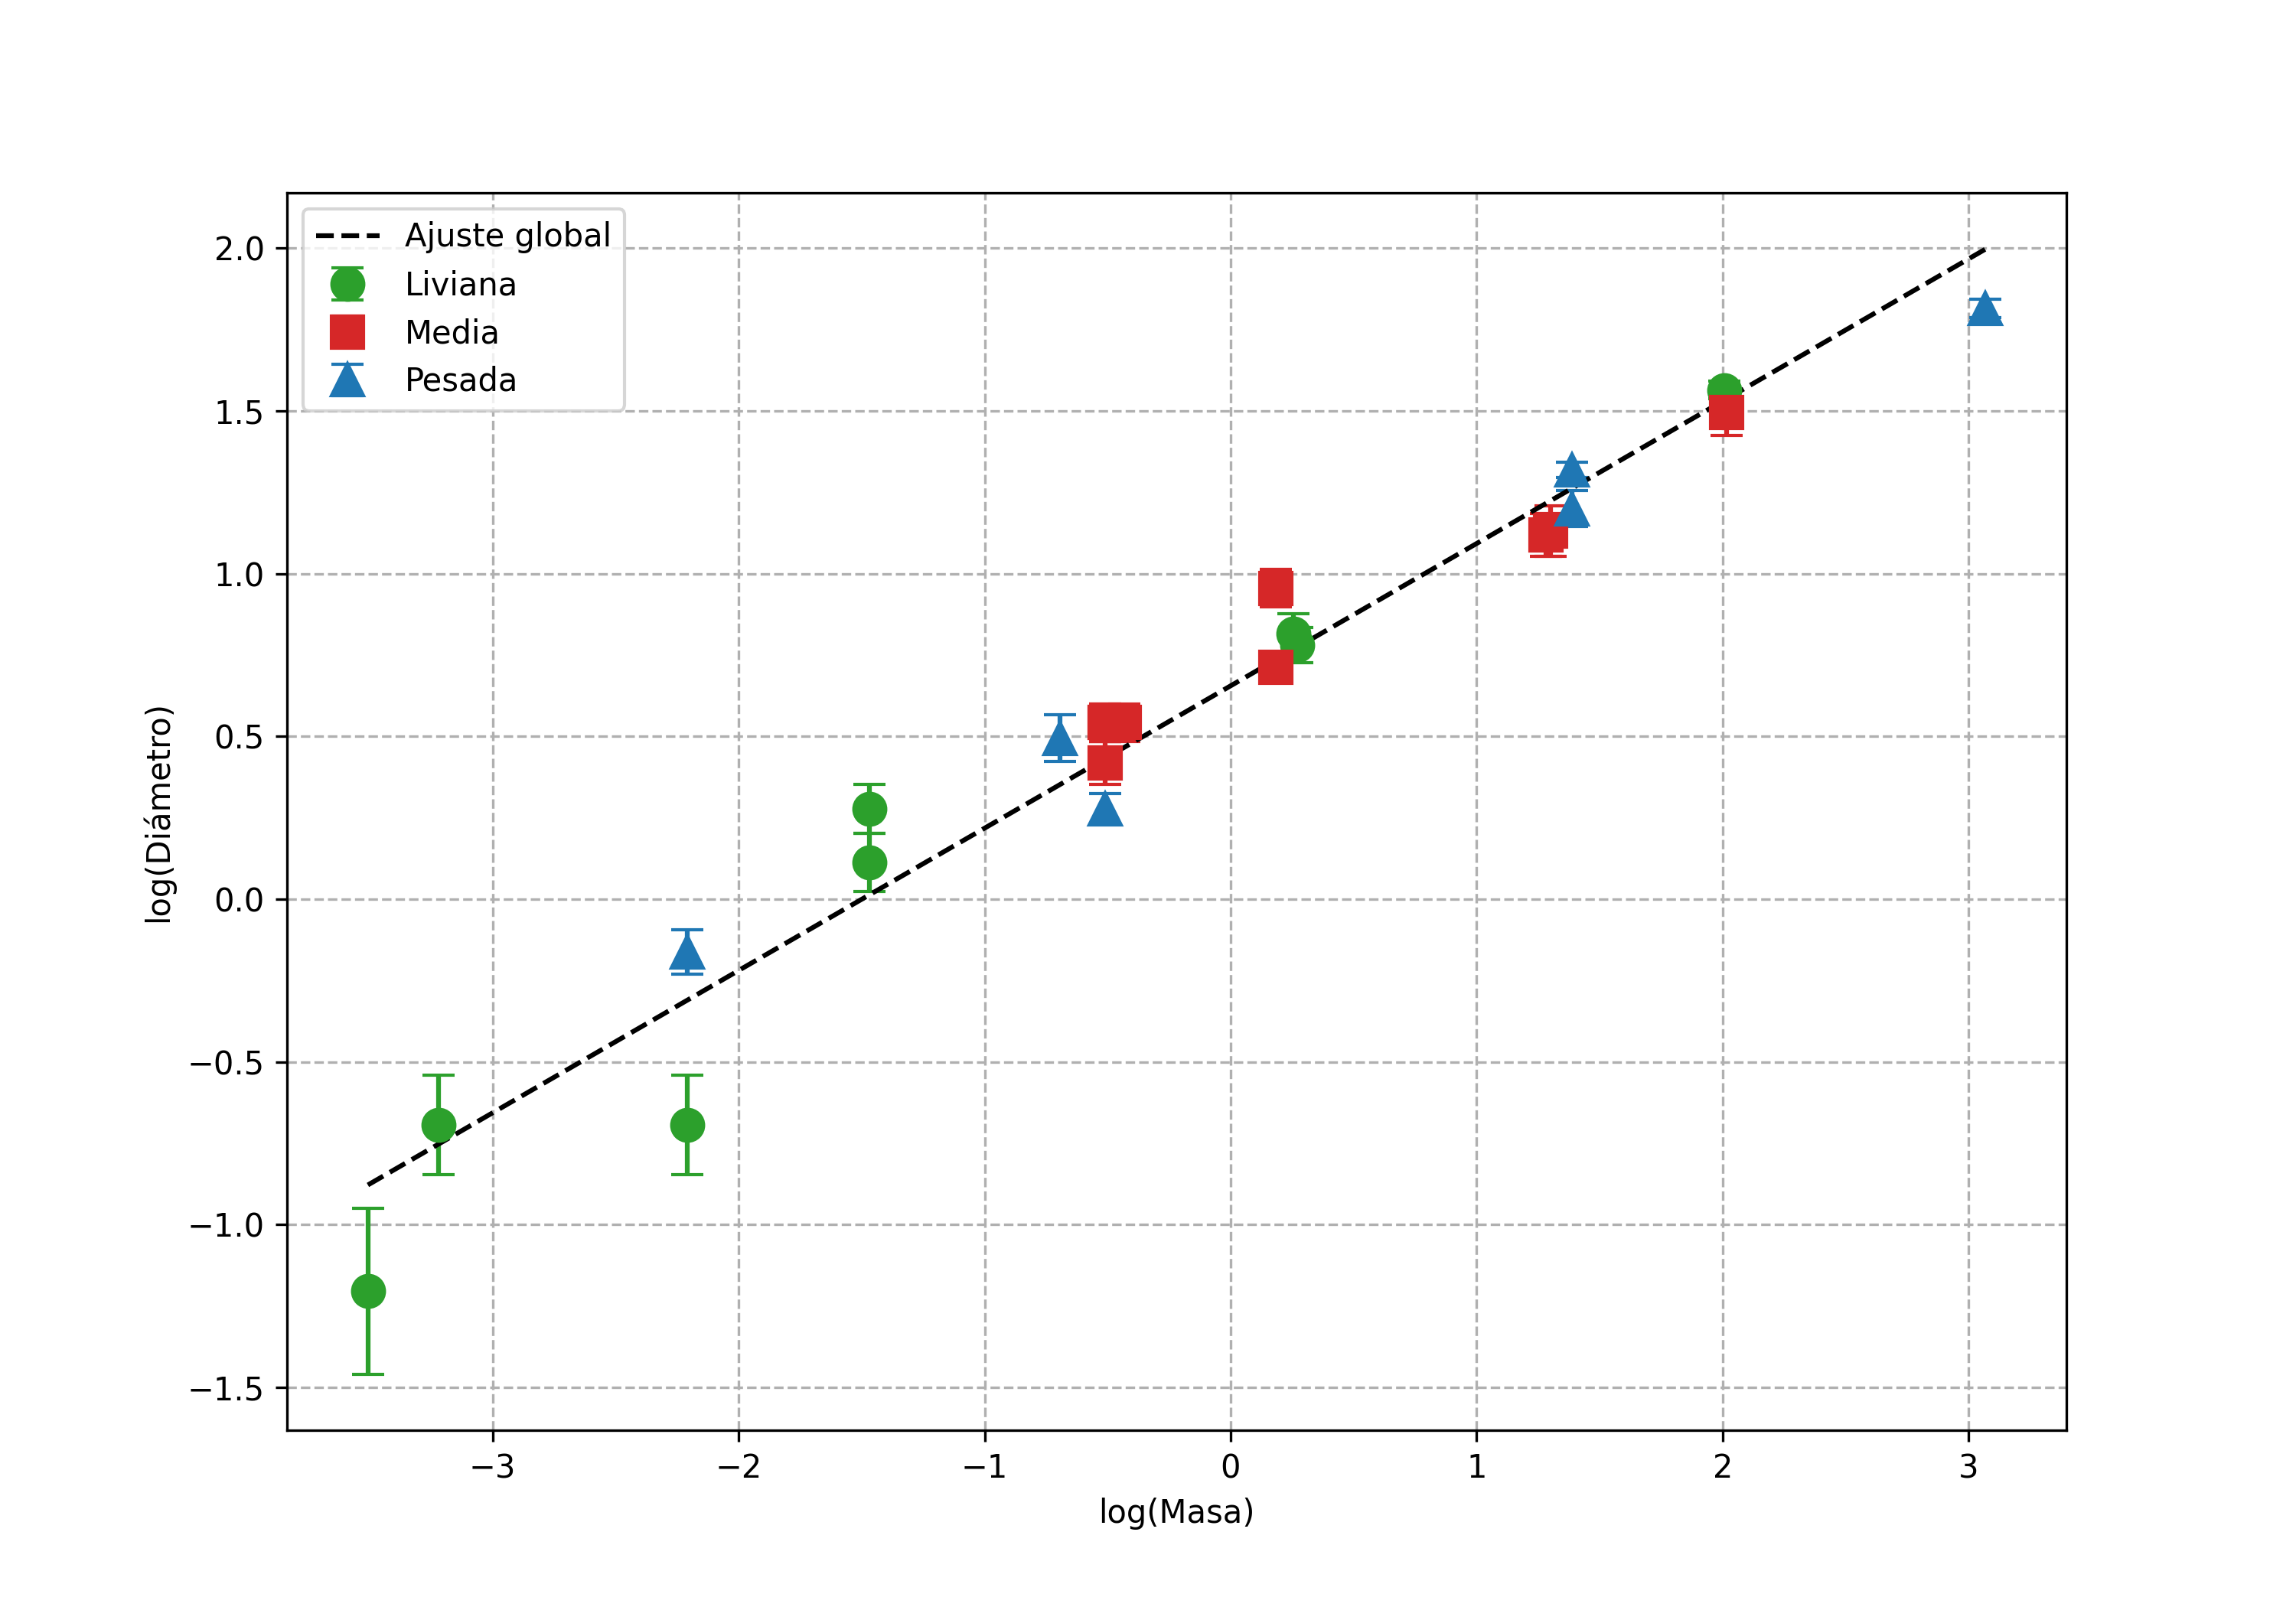
\includegraphics[width=0.45\textwidth]{loglog_diametro_vs_masa.png}
    \caption{Gráfico log-log del diámetro en función de la masa. La linealidad observada sugiere la validez del modelo de escala.}
    \label{fig:loglog}
\end{figure}

\subsection{Comparación de métodos de ajuste}

Se aplicaron dos enfoques para ajustar el modelo: un ajuste lineal en coordenadas logarítmicas, y un ajuste no lineal directo sobre los datos originales. Ambos métodos se implementaron con funciones desarrolladas en Python, como \texttt{ajuste\_lineal()} y \texttt{curve\_fit()}, incorporando las incertidumbres individuales de cada muestra.

Los resultados obtenidos con ambos métodos son consistentes, como se muestra en la Tabla~\ref{tab:ajustes}. Las diferencias entre métodos se encuentran dentro de las barras de error estimadas a partir de las matrices de covarianza.

\begin{table}[H]
\centering
\begin{tabular}{@{}lccc@{}}
\toprule
\textbf{Grupo} & \textbf{\( b \)} (log-log) & \textbf{\( b \)} (no lineal) & \textbf{\( A \)} \\
\midrule
Liviana & 0{,}481 ± 0{,}028 & 0{,}447 ± 0{,}014 & 1{,}96 ± 0{,}05 \\
Media   & 0{,}368 ± 0{,}025 & 0{,}368 ± 0{,}025 & 2{,}01 ± 0{,}04 \\
Pesada  & 0{,}388 ± 0{,}012 & 0{,}394 ± 0{,}010 & 1{,}94 ± 0{,}04 \\
\bottomrule
\end{tabular}
\caption{Parámetros obtenidos mediante ambos métodos de ajuste, según el tipo de papel.}
\label{tab:ajustes}
\end{table}

\textit{Consideración metodológica.} Como se discute en Clauset et al.~\cite{clauset}, la presencia de una recta en un gráfico log-log no constituye evidencia concluyente de una ley de potencia. Este comportamiento puede corresponder a otras distribuciones con colas pesadas. En este trabajo, se utiliza el modelo \( D = A \cdot M^b \) como una hipótesis empírica respaldada por los datos experimentales.

\subsection{Interpretación del exponente \( b \)}

El exponente \( b \) representa cómo escala el diámetro del bollo con respecto a la masa del papel. Los valores obtenidos están comprendidos entre 0,36 y 0,48. Una mayor pendiente indica que el diámetro crece más rápidamente con la masa, lo cual puede reflejar una menor eficiencia en la compactación del papel.

\begin{figure}[H]
    \centering
    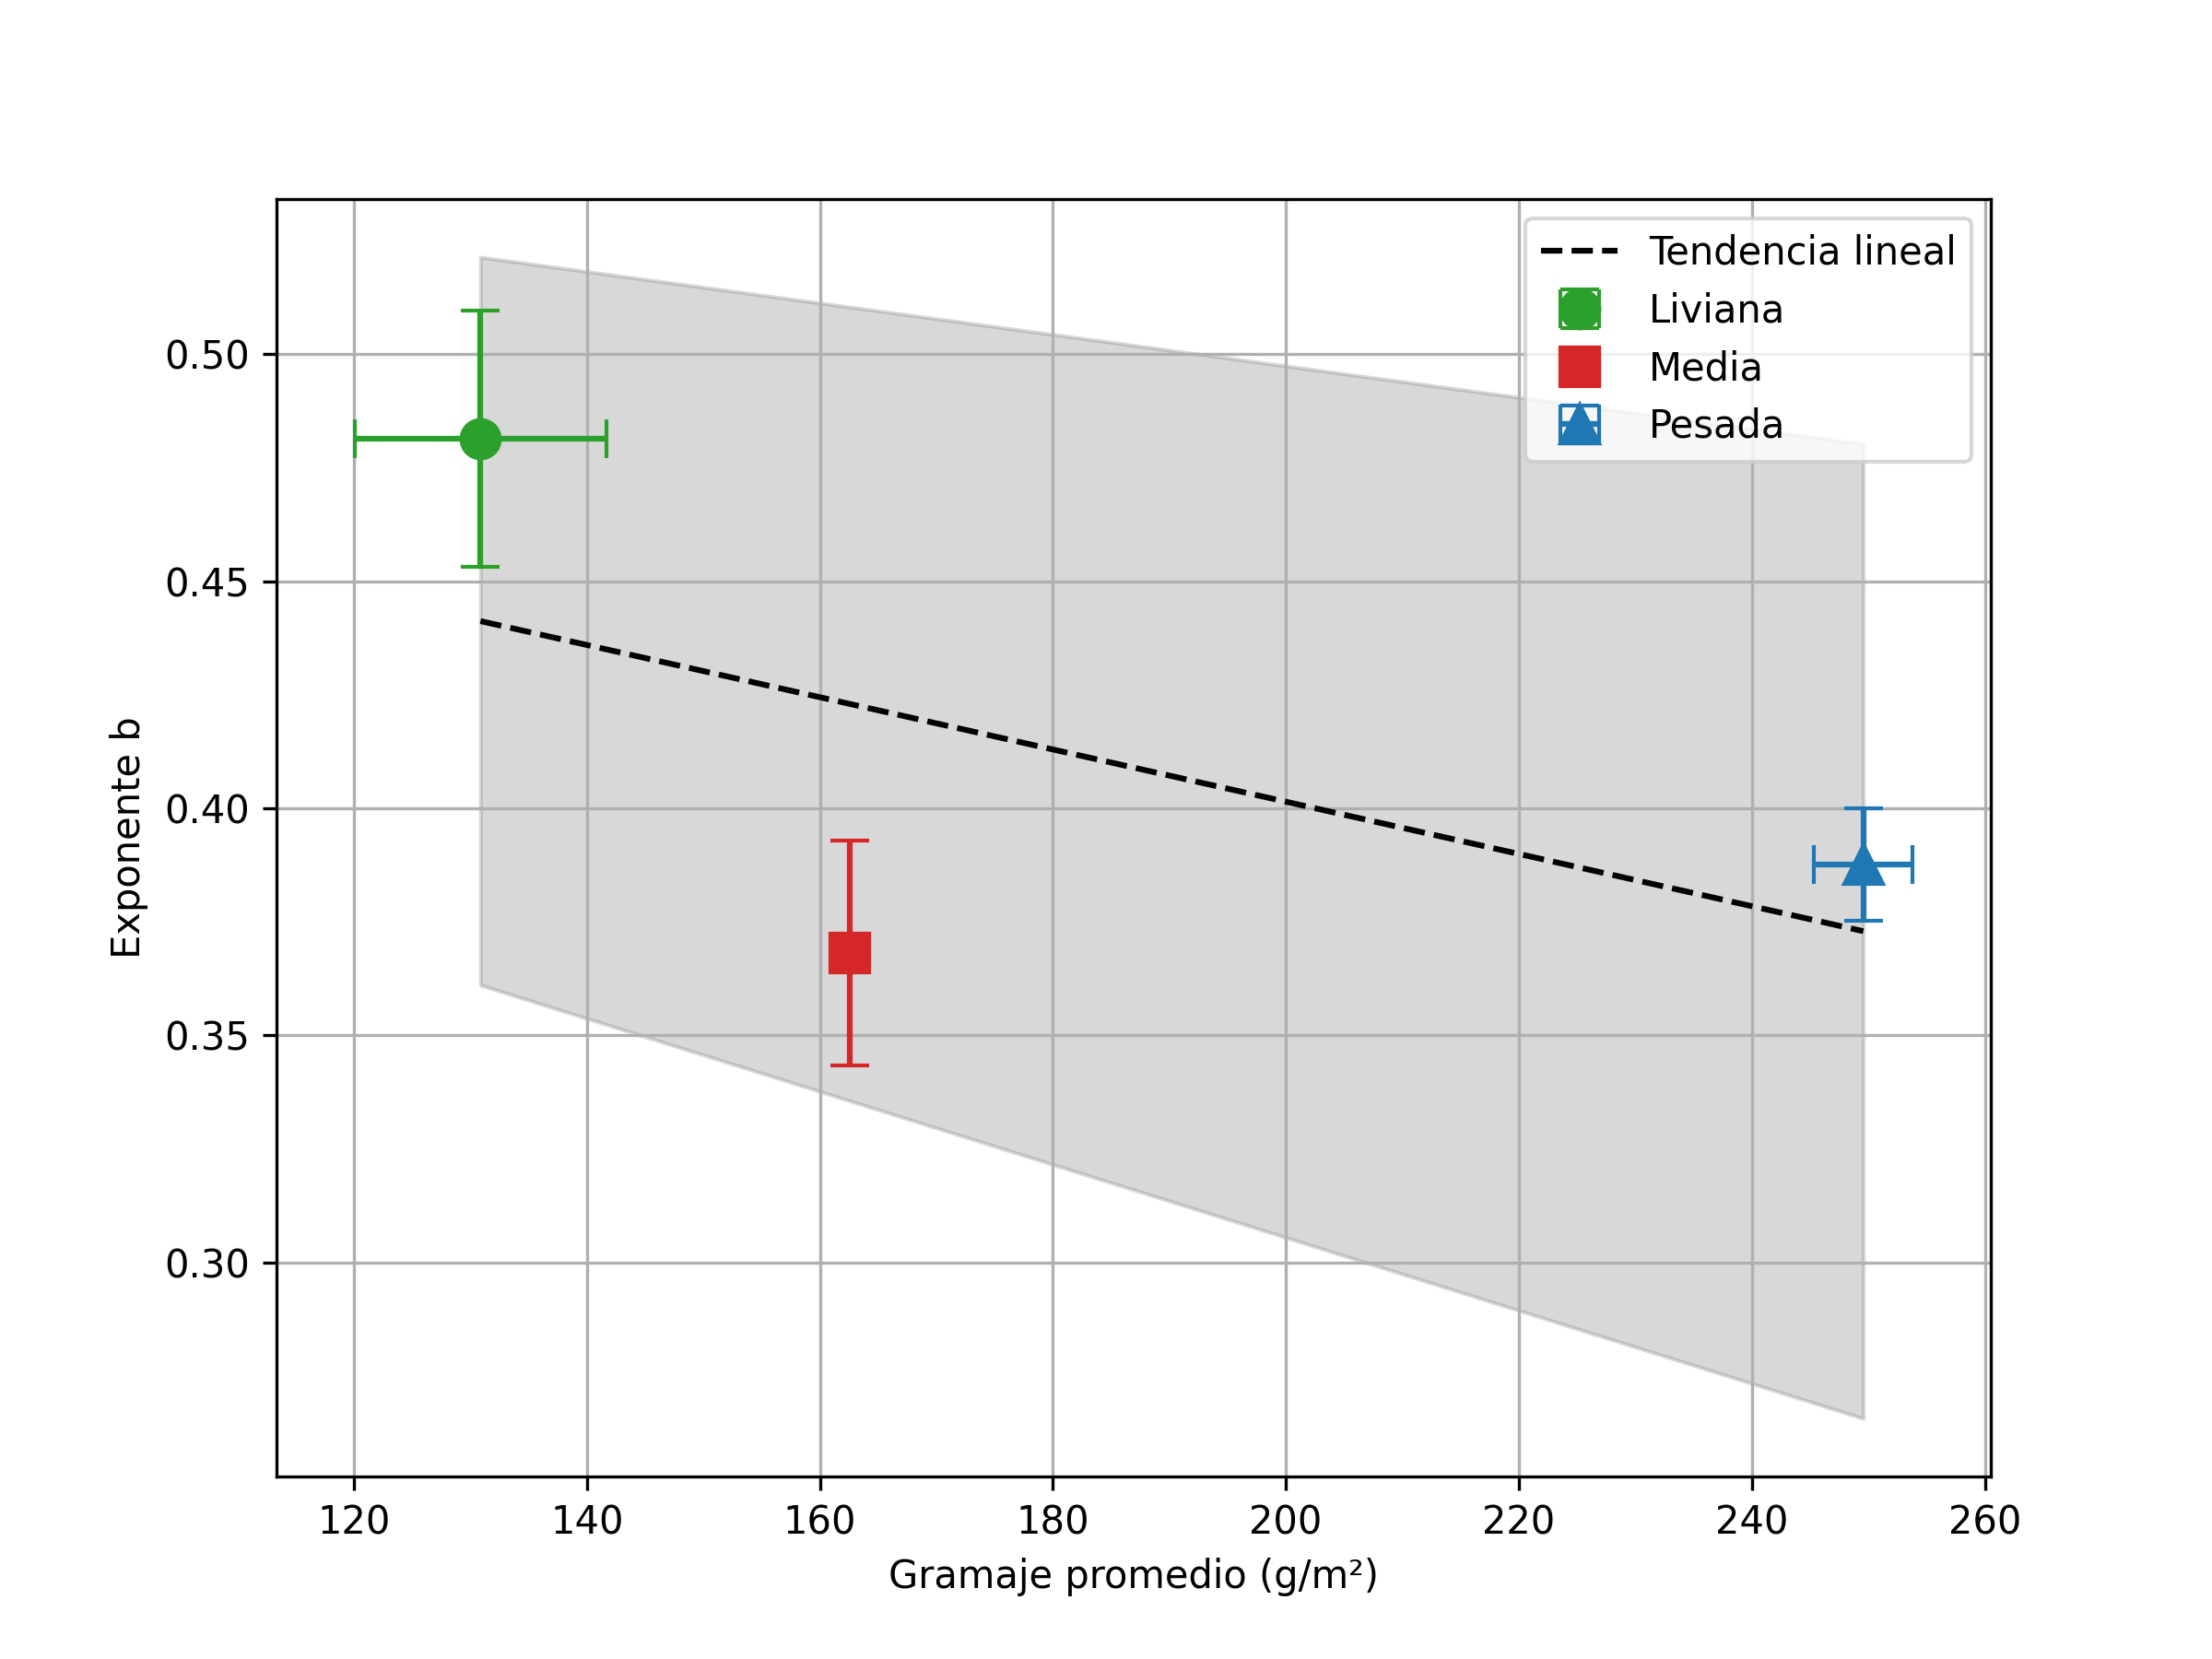
\includegraphics[width=0.45\textwidth]{b_vs_gramaje.png}
    \caption{Variación del exponente \( b \) en función del gramaje del papel. Las barras de error reflejan las incertidumbres del ajuste.}
    \label{fig:b_vs_gramaje}
\end{figure}

En la Figura~\ref{fig:b_vs_gramaje} se observa una tendencia creciente del exponente con el gramaje del papel. Esto sugiere que materiales más rígidos (mayor gramaje) presentan mayor resistencia a la compactación, generando bollos menos densos y aumentando el valor de \( b \).

\subsection{Estimación del gramaje por ajuste ortogonal}

Además del cálculo individual del gramaje mediante Ec.~\eqref{eq:gramaje}, se realizó una estimación global a partir de un ajuste lineal ortogonal del modelo \( M = G \cdot A \), utilizando la función \texttt{ajuste\_odr()}.

Este procedimiento permite considerar incertidumbres tanto en masa como en área, y evita el sesgo que se introduciría al calcular promedios individuales. Los resultados se resumen en la Tabla~\ref{tab:gramaje}.

\begin{table}[H]
\centering
\begin{tabular}{@{}lcc@{}}
\toprule
\textbf{Grupo} & \( G \) (g/m²) & \( \Delta G \) \\
\midrule
Liviana & 83{,}9 & 0{,}6 \\
Media   & 165{,}5 & 0{,}5 \\
Pesada  & 250{,}7 & 4{,}3 \\
\bottomrule
\end{tabular}
\caption{Estimación del gramaje mediante ajuste ODR para cada tipo de papel.}
\label{tab:gramaje}
\end{table}

Estos valores son coherentes con las categorías comerciales de papel, y presentan una dispersión menor que la obtenida por cálculos individuales.

\subsection{Limitaciones del modelo}

\begin{itemize}
    \item La forma esférica asumida para los bollos (ver Ec.~\eqref{eq:volumen}) es una simplificación que introduce error sistemático.
    \item La técnica de compactación fue manual y no cuantificada, lo que puede introducir variabilidad entre muestras.
    \item El rango de masas estudiado es limitado, lo cual restringe la generalización de los resultados.
    \item Se asumió homogeneidad en el papel, sin análisis estructurales adicionales (como microscopía o mediciones de rigidez).
\end{itemize}

\section{Conclusión}

Este estudio tuvo como objetivo investigar la relación entre el diámetro de bollos de papel y la masa de la hoja utilizada, evaluando la hipótesis de una ley de escala del tipo \( D = A \cdot M^b \). Se seleccionaron tres tipos de papel con gramajes distintos y se realizaron mediciones sistemáticas de sus dimensiones, masas y los diámetros de los bollos formados. El análisis experimental incluyó la propagación de incertidumbres y ajustes tanto en coordenadas log-log como no lineales.

Los resultados muestran evidencia empírica clara de una relación de tipo potencia entre el diámetro del bollo y la masa del papel en cada grupo estudiado (Figuras~\ref{fig:diametro_vs_masa} y~\ref{fig:loglog}). La correspondencia entre los datos y el modelo sugiere que la ley de escala propuesta describe adecuadamente el comportamiento del sistema bajo las condiciones experimentales consideradas.

Un hallazgo importante fue la variación del exponente \( b \) según el gramaje del papel (Tabla~\ref{tab:ajustes} y Figura~\ref{fig:b_vs_gramaje}). Se observó una tendencia creciente de \( b \) con el aumento del gramaje, lo que indica que propiedades estructurales del material, como la rigidez y la densidad superficial, influyen directamente en el proceso de compactación. Esta variación evidencia que el exponente no es universal, sino que depende de características intrínsecas del material, un aspecto clave al aplicar leyes de escala a sistemas físicos reales.

Asimismo, la estimación del gramaje mediante un ajuste ortogonal del modelo \( M = G \cdot A \) arrojó valores consistentes con las categorías de papel utilizadas. Este método, al considerar incertidumbres en ambas variables, resultó más robusto que los cálculos individuales y reforzó la validez global del análisis experimental.

Desde el punto de vista metodológico, el trabajo integró herramientas analíticas, computacionales y estadísticas para el tratamiento riguroso de los datos, desde la propagación de errores hasta los ajustes con incertidumbre. Esta aproximación permitió evaluar con precisión la consistencia del modelo y su aplicabilidad en un contexto físico tangible.

Si bien los resultados respaldan el uso del modelo \( D = A \cdot M^b \) como una ley de escala válida en este sistema, no se afirma su carácter universal. Como advierten Clauset et al.~\cite{clauset}, la linealidad en coordenadas logarítmicas no constituye por sí sola una prueba concluyente de una ley de potencia. No obstante, en el marco de este estudio, el modelo se mostró coherente, reproducible y físicamente significativo.

En conjunto, este trabajo demuestra que un fenómeno cotidiano puede analizarse con rigor científico, revelando dinámicas complejas en sistemas aparentemente simples. La dependencia del exponente de escala con el gramaje abre la puerta a futuras investigaciones sobre la influencia de otras propiedades del papel —como el espesor, la elasticidad o la estructura interna— en el comportamiento geométrico y mecánico de materiales comprimidos.


\appendix
\section{Código fuente y procesamiento de datos}

Todo el procesamiento de datos experimentales, el ajuste de modelos y la generación de gráficos fue realizado mediante un script en Python. El código incluye funciones personalizadas para:

\begin{itemize}
    \item Cálculo de magnitudes derivadas con propagación de incertidumbres.
    \item Ajustes lineales y no lineales ponderados.
    \item Ajuste ortogonal (ODR) para estimar el gramaje.
    \item Automatización de gráficos y exportación de resultados.
\end{itemize}

El código se encuentra disponible públicamente en el siguiente repositorio de GitHub:

\begin{center}
\href{https://github.com/HowlingPython/Informe_1_Fisica.git}{\texttt{github.com/HowlingPython/Informe\_1\_Fisica}}
\end{center}

El script principal se llama:

\begin{itemize}
    \item \texttt{Lopez\_Moroni\_Tornielli\_Fisica\_TP1.py}
\end{itemize}

Cada función está documentada y se encuentra organizada por bloques temáticos (análisis de muestras, ajustes, gráficos, exportación de datos, etc.), lo que facilita su lectura y reutilización.

\printbibliography
\end{document}